\section{PRELIMINARIES}
In this section we introduce the definition of \BCNs\ and their algebraic form as well as the four existing kinds of observability of {\em BCNs}.



\subsection{Boolean Control Networks}

A Boolean control network can be described as a directed graph together with logical equations to describe the updating rules of the nodes in the graph, the definition of {\em BCN} is as follows. 

\begin{definition}
(\cite{Ideker2001A}) A \BCN\ consists of input-nodes, state-nodes, output-nodes, and directed edges which connect nodes. A node in \BCN\ can take a logic value from $\{0,1\}$ at a discrete time $0, 1, 2,\ldots$. For one directed edge from a state node (or an input node) $s_1$ (or $i$) to a state node $s_2$ means that the logic value of $s_2$ at time step $t+1$ is affected by the value of $s_1$ (or $i$)  at time step $t$. For one directed edge from a state node $s_1$ to a output node $o_1$ means that the logic value of $o_1$ at time step $t$ is affected by the value of $s_1$  at time step $t$. 
\end{definition}


Note that one can only know whether or not a node is affected by another node from the network graph. Different \BCNs\ may have the same structure, in order to determine a \BCN\ uniquely, logical equations are also needed to describe the specific updating rules of {\em BCNs}.

 
 \begin{figure}[thpb]
      \centering
      \framebox{\parbox{3in}{
		\centerline{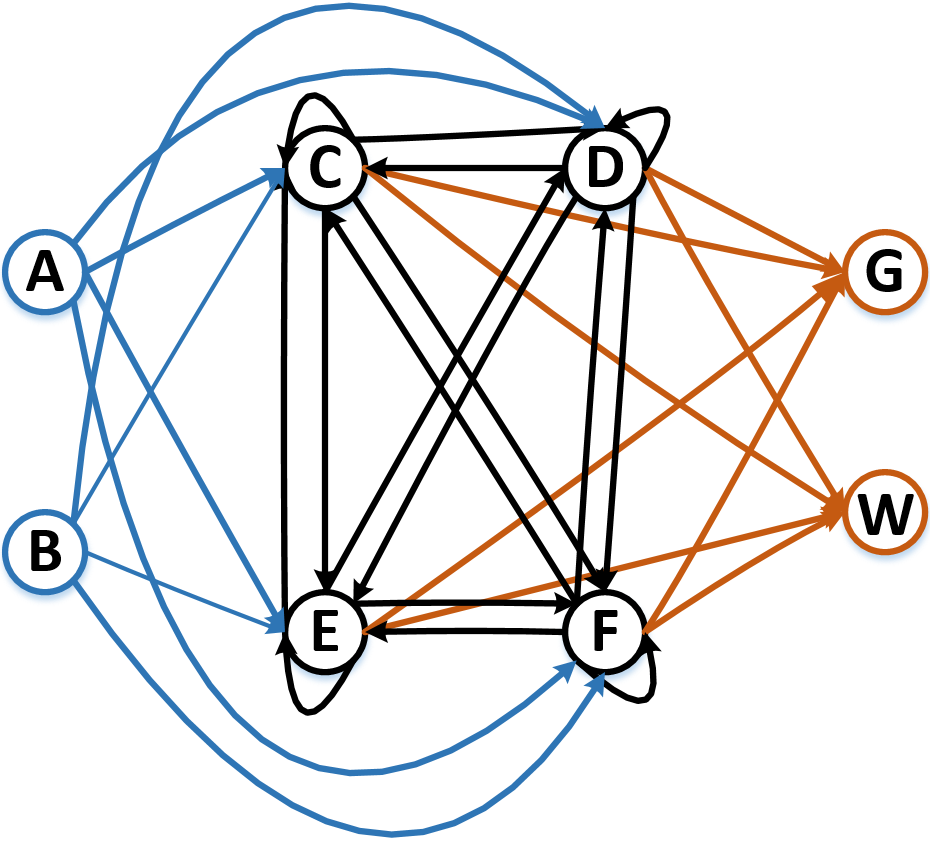
\includegraphics[scale=0.23]{figures/Fig1.png}}
	}}
      
      \caption{A Boolean control network with two input-nodes $A$ and $B$, four state-nodes $C$, $D$, $E$ and $F$, and two output-nodes $G$, $W$. We use blue, black and orange, to distinguish three kinds of nodes and three kinds of edges.}
      \label{fig:1}
  \end{figure}

To better illustrate the concept of {\em BCNs}, we give a simple example to describe it.

\begin{example}
	In Fig.\ref{fig:1} we have a \BCN\ with two input-nodes $A$ and $B$, four state-nodes $C$, $D$, $E$ and $F$, and two output-nodes $G$, $W$. The \BCN\ is shown in Fig.\ref{fig:1}, and the updating rules of this \BCN\ are described as truth table Fig.\ref{fig:2}. The reason why we use truth table to describe the updating rules of the \BCN\ is that this form of updating rules will be more convenient for \BCN\ to convert into its aglebraic form. What's more, for instance, we can know the updating rule of state-node $G$ from the truth table,
	\[G(t)=C(t)\wedge \neg(\neg{D(t)}\wedge \neg E(t)\wedge \neg F(t))\]
	
	For convenience, we will use this example in the whole paper to explain various concepts we introduce.
  \begin{figure}[thpb]
      \centering
      \framebox{\parbox{3in}{
		\centerline{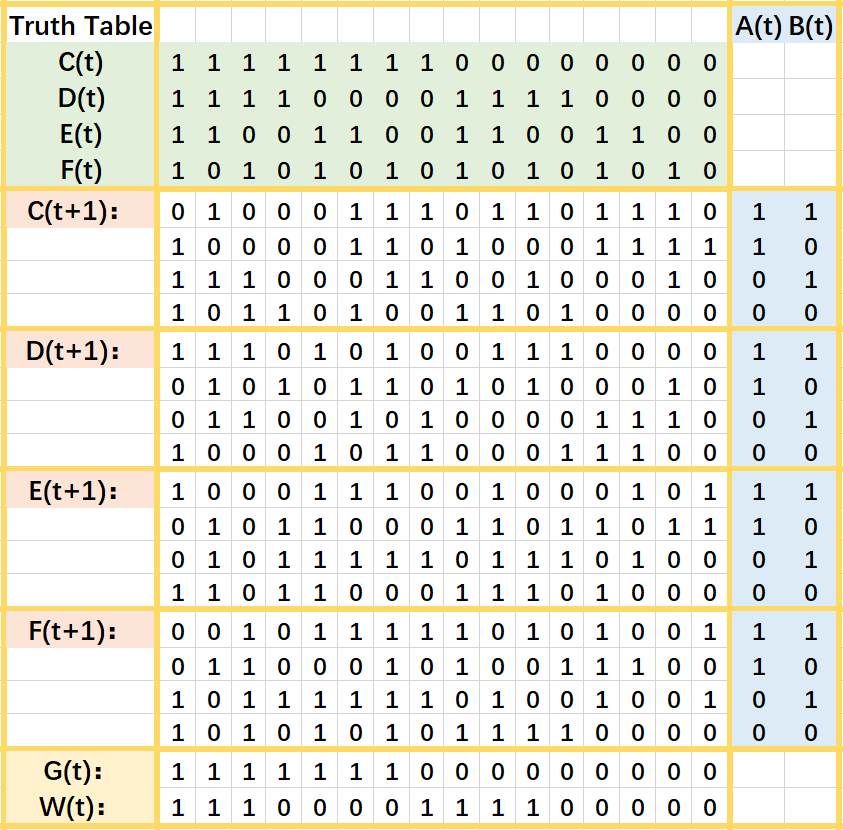
\includegraphics[scale=0.26]{figures/Fig21.png}}
	}}
      
      \caption{The truth table which describe the updating rules of the \BCN\ shown in {\em Fig.\ref{fig:1}}.}
      \label{fig:2}
   \end{figure}
\end{example}   


%==============================================================================================================
\subsection{The Algebraic Forms of BCNs}
To better illustrate the concept of algebraic forms, in this paper, we investigate the following \BCN\ assumes to has $n$ state-nodes, $m$ input-nodes and $q$ output-nodes. Then the updating rules of the \BCN\ can be described as following formulas:
\begin{equation}
\begin{split}
s(t+1)=&f(i(t),s(t))\\
o(t)=&h(s(t))
\end{split}
\label{equ:1}
\end{equation}
$s(t)\in \mathbb{B}^n$ are state-nodes; $i(t)\in \mathbb{B}^m$ are input-nodes; $o(t)\in \mathbb{B}^q$ are output-nodes; $f:\mathbb{B}^{n+m}\mapsto \mathbb{B}^n$ and $h:\mathbb{B}^n\mapsto \mathbb{B}^q$ are logical functions that represent the updating rules of {\em BCNs}. Where $\mathbb{B}$ : the set $\{0,1\}$; $t=0,1,\ldots$ represents the discrete time. 

Therefore in the previously mentioned example, we have $C(t), D(t), E(t), F(t)\in s(t)$; $A(t), B(t)\in i(t)$ and $G(t), W(t)\in o(t)$; $n=4$, $m=2$ and $q=2$; $f$ and $h$ are described in the truth table ({\em Fig.\ref{fig:2}}). 

The {\em STP} of matrices can be used to represent the algebraic forms of {\em BCNs} \cite{cheng2009controllability}, the definition of {\em STP} is as follows.

\begin{definition}[STP] 
	\cite{Cheng2011Analysis} Let $X\in\mathbb{R}_{m\times n}$, $Y\in\mathbb{R}_{p\times q}$ and $\alpha=lcm(n,p)$ be the least common multiple of $n$ and $p$. The STP of $X$ and $Y$ is defined as \[X\ltimes Y=(X\otimes I_{\alpha/n})(Y\otimes I_{\alpha/p}),\] where $\otimes$ denotes the Kronecker product. 
\end{definition}

After introduce the definition of {\em STP} of matrices,  we introduce some related notations at first \cite{Zhang2016Observability}:
\begin{itemize}
  \item $\delta^i_n$: the $i$-th column of the identity matrix $I_n$;
  \item $\Delta_n$: the set $\{\delta^1_n,\ldots,\delta^n_n \}$; 
  \item $\delta_n \left[i_1,\ldots,i_s\right]$: $\left[\delta^{i_1}_n,\ldots,\delta^{i_s}_n\right]\left(i_1,\ldots,i_s\in\left\{1,2,\ldots,n\right\}\right)$ the logical matrix;
  \item  $L_{n\times s}$: the set of $n\times s$ logical matrices.
\end{itemize}


Using {\em STP} of matrices, the formula (\ref{equ:1}) can be quivalently represented in the following algebraic form:
\begin{equation}
\begin{split}
s(t+1)=&L\ltimes{i(t)}\ltimes{s(t)}\\
o(t)=&H\ltimes{s(t)}
\end{split}
\label{equ:2}
\end{equation}
where $s(t)\in\Delta_N$, $i(t)\in\Delta_M$, and  $o(t)\in\Delta_Q$ denote the states, inputs and outputs respectively the same as in {\em (\ref{equ:1})}, but they are with vector forms; $L\in L_{N\times\left(NM\right)}$; $H\in L_{Q\times N}$ denote the relation matrices; that $N=2^n$, $M=2^m$, and $Q=2^q$. Since {\em STP} keeps most properties of the conventional product \cite{Cheng2011Analysis}, the associative law, the distributive law, etc., we usually omit the symbol ``$\ltimes$'' hereinafter. For instance, the 
formula ``$s(t+1)=L\ltimes{i(t)}\ltimes{s(t)}$'' can be written as ``$s(t+1)=L{i(t)}{s(t)}$''.

To construct algebraic form (\ref{equ:2}) we give a mapping $\tau:\{0,1\}\mapsto \{\delta_2^1, \delta_2^2\}$ where $\tau(0)=\delta_2^2$, $\tau(1)= \delta_2^1$. 
%each logical value a vector form as: $1 \scriptsize{\sim} \delta_2^1$, $0 \scriptsize{\sim} \delta_2^2$. 
Therefore, the logical variable $A(t)$ takes value from these two vectors, i.e., $A(t)\in \{\delta_2^1, \delta_2^2\}$. Using the {\em STP} of matrices, we have 
\[i(t)=i_1(t){\ldots}i_m(t);\] 
\[s(t)=s_1(t){\ldots}s_n(t);\] 
\[o(t)=o_1(t){\ldots}o_q(t).\] 
And according to \cite{Cheng2003Semi}, each logical function $f_p$ of state-nodes can be found in the updating rules (\ref{equ:1}). The form of  $f_p$ as:
\[f_p(i_1(t),\ldots,i_m(t),s_1(t),\ldots,s_n(t))\] 
and there exists a structure matrix $L_p\in L_{2\times {NM}}$ such that
\begin{equation}
\begin{split}
\tau(f_p(i_1(t),\ldots,i_m(t),s_1(t),\ldots,s_n(t)))= L_pi(t)s(t)
\end{split}
\end{equation}
%where the left side of equation calculate the truth value and the right side of equation calculate the vector in $\{\delta_2^1, \delta_2^2\}$. 
For state-nodes $s_1,\ldots,s_n$, we have $n$ logical matrices $L_1,\ldots,L_n$ for them, respectively. 
%We have that
%when\\
If for each state-node $s_p$ the logical matrix has form
\[L_p=[\delta_2^{p_1},\ldots,\delta_2^{p_{NM}}],\] 
then we have that %for the set of all state-nodes $s(t)$ the logical matrix 
\[L=[\delta_N^{R_1},\ldots,\delta_N^{R_{NM}}]\]  where 
\[\delta_N^{R_1}=\delta_2^{1_1}\ldots\delta_2^{n_1};\ldots; \delta_N^{R_{NM}}=\delta_2^{1_{NM}}\ldots\delta_2^{n_{NM}}.\] 
%then 
By this relationship we can construct the $L$ for the algebraic forms of {\em BCNs}. What's more we can also construct the logical matrix $H$ in the similar way.

For instance, the \BCN\ whose structure is depicted in Fig.\ref{fig:1}, and the updating rules of this \BCN\ is described as truth table in Fig.\ref{fig:2}. We have that the updating rules of this \BCN\ can be represented with the algebraic form:
\begin{equation}
\begin{split}
s(t+1) =&\delta_{16}[\alpha]i(t)s(t)\\
o(t) =&\delta_4[\beta]s(t)\\
\end{split}
\end{equation}
where $\alpha=\{10,4,11,16,9,5,1, 7,15,2,3,12,7,6,8,13,8,9,\\15,10,14,4,3,16,1,14,12,13,5,7,2,6,7,2,3,13,13,9,5,1,\\16,13 ,6,14,11,10,4,15,1,14 ,7,6,9 ,8,11,12,5,5,13,3,10,\\12,16,16\}$, $\beta=\{1,1,1,2,2,2,2,3,3,3,3,4,4,4,4,4\}$, $t\in \mathbb{N}$, $s\in \Delta_{16}$, $i\in \Delta_4$ and $o\in \Delta_4$.
\subsection{Four Existing Observability of BCNs}
In this section we introduce four existing kinds of observability of {\em BCNs}. Let $\Delta_N$, $\Delta_M$, $\Delta_Q$ be three alphabets, for all $s_0\in \Delta_N$ and all $p\in \mathbb{Z}_+$; $\infty$ is the infinite natural numbers. In order to introduce four existing kinds of observability of {\em BCNs}, we define the mappings \cite{Zhang2016Observability}:
\begin{equation}
\begin{split}
L^p_{s_0} &: (\Delta_M)^p\mapsto(\Delta_N)^p, u_0\ldots u_{p-1} \mapsto s_1 \ldots\, s_p\\
L^{\infty}_{s_0} &: (\Delta_M)^{\infty}\mapsto(\Delta_N)^{\infty}, u_0 u_1 \ldots  \mapsto s_1 s_2 \ldots
\end{split}
\end{equation}
\begin{equation}
\begin{split}
(HL)^p_{s_0} &: (\Delta_M)^p\mapsto(\Delta_Q)^p, u_0\ldots u_{p-1} \mapsto o_1\ldots\, o_p\\
(HL)^{\infty}_{s_0} &: (\Delta_M)^{\infty}\mapsto(\Delta_Q)^{\infty}, u_0 u_1 \ldots  \mapsto o_1 o_2\ldots
\end{split}
\end{equation}

For all  $p\in \mathbb{Z}_+$, all $U=u_1 \ldots u_p \in(\Delta_M)^p$, and all $1\ge i \ge j \ge |U|$, we use U[i,j] to denote the word $u_i \ldots u_j$ as a input sequence. Then four existing kinds of observability of BCNs can be define as: 
\begin{definition}
The first kind of observability is that, \BCN\ is called observable, if for every initial state $s_0 \in \Delta_N$, there exists an input sequence $U\in(\Delta_M)^p$ for some $p\in \mathbb{Z}_+$ such that for all states $s_0\neq {s'}_0\in \Delta_N$, $Hs_0=H{s'}_0$ implies $(HL)^p_{s_0}(U)\neq (HL)^p_{{s'}_0}(U)$ \cite{cheng2009controllability}.
\end{definition}

Hence the first observability means that if a \BCN\ is observable then every initial state of the \BCN\ can be determined by an input sequence. But we can only use the corresponding input sequence of a state to check whether this state is the initial state of the {\em BCN} or not.
\begin{definition}
	The second kind of observability is that a \BCN\ is called observable if for any distinct states $s_0$, ${s'}_0 \in \Delta_N$, there exists an input sequence $U\in(\Delta_M)^p$ for some $p\in \mathbb{Z}_+$, such that $Hs_0=H{s'}_0$ implies $(HL)^p_{s_0}(U)\neq (HL)^p_{{s'}_0}(U)$ \cite{Zhao2010Input}.
\end{definition}

The second observability means that a \BCN\ is called observable if for every two distinct initial states of the {\em BCN}, there exists an input sequence which can distinguish them. 
\begin{definition}
	The third kind of observability is that, a \BCN\ is called observable, if there exists an input sequence $U\in(\Delta_M)^p$ for some $p\in \mathbb{Z}_+$, such that for any distinct states $s_0$, ${s'}_0 \in \Delta_N$, $Hs_0=H{s'}_0$ implies $(HL)^p_{s_0}(U)\neq (HL)^p_{{s'}_0}(U)$ \cite{Cheng2011Identification}.
\end{definition}

The third observability means that a \BCN\ is called observable if there is an input sequence that determines the initial state of the {\em BCN}.
\begin{definition}
	The fourth kind of observability is that, \BCN\ is called observable, if for any distinct states $s_0$, ${s'}_0 \in \Delta_N$, for any input sequence $U\in(\Delta_M)^{\infty}$, $Hs_0=H{s'}_0$ implies $(HL)^{\infty}_{s_0}(U)\neq (HL)^{\infty}_{{s'}_0}(U)$ \cite{Fornasini2013Observability}.
\end{definition}

The fourth observability means that a \BCN\ is called observable if every sufficient long input sequence can determine the initial state of the {\em BCN}.

Then from the definitions of  four existing kinds of observability, we know that \cite{Zhang2016Observability}:
\begin{itemize}
  \item the first one implies the second one;
  \item the third one implies the second one and first one;
  \item the fourth one implies the third one, second one and first one.
\end{itemize} 
%, when we don't presuppose the initial state of {\em BCNs}
 And we can't use the first one and second one to determine the initial state of {\em BCNs} which can be checked at most once. For example, in the first kind observability we need to assume the initial state of a {\em BCN}, and then check it by corresponding input sequence of this state. If the state we assume is correct, then we can determine the initial state. But if the the assumption is not correct, we can't determine the initial state of the {\em BCN}. Therefore we need to check the \BCN\ again and again untill we can determine the initial state of it. However we can use the third existing observability and fourth existing observability to determine the initial state of {\em BCNs} in one time. And we need not to presuppose the initial state of {\em BCNs} when we use the third observability and fourth observability. But the requirements for {\em BCNs} are very harsh when we use the third observability and fourth observability. With these disadvantages of four existing observabilities, we propose the online observability of {\em BCNs} to solve this problem.
 \subsubsection*{Problem}
Finding the necessary and sufficient condition of determine the initial state of {\em BCNs} in one time and without presupposing the range of its initial state.